\subsection{NLoS branch}
\label{sec:nlos_branch_detail}

The NLoS path-loss branch is a hybrid model built in four stages.

\subsubsection{Stage 1: raw NLoS propagation prior}

\paragraph{COST-231 term.}
\begin{equation}
\mathrm{PL}_{\mathrm{COST231}}(x) = 46.3 + 33.9\log_{10}(f_{\mathrm{MHz}}) - 13.82\log_{10}(h_{\mathrm{tx}}) - a(h_{\mathrm{rx}}) + \left(44.9 - 6.55\log_{10}(h_{\mathrm{tx}})\right)\log_{10}(d_{\mathrm{km}}) + 3
\label{eq:cost231}
\end{equation}
where $d_{\mathrm{km}} = d_{2D}(x)/1000$ and the mobile antenna correction factor for large cities is:
\begin{equation}
a(h_{\mathrm{rx}}) = 3.2(\log_{10}(11.75\,h_{\mathrm{rx}}))^2 - 4.97
\end{equation}

\paragraph{Elevation-aware UAV envelope.}
\begin{equation}
\mathrm{PL}_{\mathrm{A2G,NLoS}}(x) = \lambda_0(h_{\mathrm{tx}}, f) + \beta_{\mathrm{NLoS}} + A_{\mathrm{NLoS}}\exp\!\left(-\frac{90-\theta^\circ(x)}{\tau_{\mathrm{NLoS}}}\right)
\label{eq:a2g_nlos}
\end{equation}
where $\lambda_0(h_{\mathrm{tx}}, f) = 20\log_{10}\!\left(\frac{4\pi h_{\mathrm{tx}} f}{c}\right)$, with fitted constants $\beta_{\mathrm{NLoS}} = -16.16$~dB, $A_{\mathrm{NLoS}} = 12.0436$, $\tau_{\mathrm{NLoS}} = 7.52^\circ$.

The raw NLoS prior takes the conservative (higher) of the two estimates:
\begin{equation}
\mathrm{PL}_{\mathrm{NLoS,raw}}(x) = \max\!\left(\mathrm{PL}_{\mathrm{COST231}}(x),\,\mathrm{PL}_{\mathrm{A2G,NLoS}}(x)\right)
\label{eq:nlos_raw}
\end{equation}

The full raw prior blends LoS and NLoS estimates using the LoS mask $m_{\mathrm{LoS}}(x) \in [0,1]$:
\begin{equation}
\mathrm{PL}^{(0)}(x) = m_{\mathrm{LoS}}(x)\,\mathrm{PL}_{\mathrm{LoS,blend}}(x) + \left(1-m_{\mathrm{LoS}}(x)\right)\mathrm{PL}_{\mathrm{NLoS,raw}}(x)
\label{eq:pl0}
\end{equation}
with $\mathrm{PL}_{\mathrm{LoS,blend}}(x) = 0.7\,\mathrm{PL}_{\mathrm{LoS,path}}(x) + 0.3\min\!\left(\mathrm{PL}_{\mathrm{LoS,path}}(x),\,\mathrm{PL}_{\mathrm{A2G,LoS}}(x)\right)$.

\subsubsection{Stage 2: map-derived morphology features}

A 15-element feature vector is computed from $\mathrm{PL}^{(0)}(x)$ and the map topology:
\begin{equation}
\textbf{x}_{78}(x) = \begin{bmatrix} \mathrm{PL}^{(0)}(x)^2,\ \mathrm{PL}^{(0)}(x),\ \log(1+d_{2D}),\ \rho_{15},\ \rho_{41},\ h_{15},\ h_{41},\ \rho_{41}\log(1+d_{2D}),\ n_{15},\ n_{41},\ n_{41}\log(1+d_{2D}),\ \sigma_{\mathrm{shadow}},\ \theta_{\mathrm{norm}},\ n_{41}\theta_{\mathrm{norm}},\ 1 \end{bmatrix}^\top
\label{eq:x78}
\end{equation}

The multiscale features use the 2D box-mean operator with window sizes $k \in \{15, 41\}$ pixels (corresponding to $\sim$15 m and $\sim$41 m neighborhoods at 1 m/pixel):
\begin{equation}
\mathrm{BoxMean}_k(f)(i,j) = \frac{1}{k^2}\sum_{i'=i-p}^{i+p}\sum_{j'=j-p}^{j+p} f_{\mathrm{padded}}(i',j')
\label{eq:boxmean}
\end{equation}
implemented efficiently via a 2D summed-area table (integral image).

Building density: $\rho_k(x) = \mathrm{BoxMean}_k(b(\cdot))(x)$ (fraction of building pixels in the window).

Building height: $h_k(x) = \mathrm{BoxMean}_k(\mathrm{topology}(\cdot)\,b(\cdot))(x)\,/\,H_{\mathrm{norm}}$, with $H_{\mathrm{norm}} = 90$~m.

NLoS support: $n_k(x) = \mathrm{BoxMean}_k(n_{\mathrm{raw}}(\cdot))(x)$, where $n_{\mathrm{raw}}(x) = \mathbb{1}[m_{\mathrm{LoS}}(x) \le 0.5]\cdot g(x)$.

Elevation angle: $\theta(x) = \arctan\!\left(\frac{h_{\mathrm{tx}}-h_{\mathrm{rx}}}{\max(d_{2D}(x),1)}\right)$, normalised as $\theta_{\mathrm{norm}}(x) = \mathrm{clip}(\theta^\circ(x)/90, 0, 1)$.

\subsubsection{Stage 3: regime-wise linear calibration}

The regime $r$ is identified by: coarse topology (\texttt{open\_lowrise}, \texttt{mixed\_midrise}, or \texttt{dense\_highrise}), propagation state (LoS or NLoS), and antenna height bin (\texttt{low\_ant}, \texttt{mid\_ant}, or \texttt{high\_ant}), giving up to $3 \times 2 \times 3 = 18$ regimes.

The topology class is assigned by thresholding map-level building density $\bar\rho_{\mathrm{map}}$ and mean building height $\bar h_{\mathrm{map}}$ with thresholds $d_1 = 0.12$, $d_2 = 0.28$, $h_1 = 12$~m, $h_2 = 28$~m. The antenna-height bin uses tertiles with cutoffs at 58.12 m and 103.85 m.

The calibrated prediction for regime $r$:
\begin{equation}
\widehat{\mathrm{PL}}_{r}(x) = \textbf{x}_{78}(x)^\top \textbf{w}^{78}_{r}
\label{eq:pl_cal}
\end{equation}
fitted by ordinary least squares:
\begin{equation}
\hat{\textbf{w}}^{78}_{r} = \left(\textbf{X}_r^\top \textbf{X}_r\right)^{-1}\textbf{X}_r^\top \textbf{y}_r
\label{eq:ols_closed}
\end{equation}

\subsubsection{Stage 4: region replacement and clipping}

\begin{equation}
\mathrm{PL}_{\mathrm{NLoS}}(x) = \mathrm{clip}\!\left(\textbf{x}_{78}(x)^\top \textbf{w}^{78}_{r},\;20,\;180\right)
\label{eq:pl_nlos_final}
\end{equation}

The final hybrid path-loss prior:
\begin{equation}
\mathrm{PL}_{\mathrm{prior}}(x) = \begin{cases} \mathrm{PL}_{\mathrm{LoS}}(x), & m_{\mathrm{LoS}}(x) > 0.5 \\ \mathrm{PL}_{\mathrm{NLoS}}(x), & \text{otherwise} \end{cases}
\label{eq:pl_hybrid}
\end{equation}

\subsection{Try 78 results}

\begin{table}[H]
\centering
\caption{Try 78 pixel-weighted RMSE (dB) on the evaluation split.}
\label{tab:try78_rmse}
\begin{tabular}{lcc}
\toprule
Model & RMSE (dB) & Role in Try 80\\
\midrule
FSPL (LoS only)            & 3.9540 & ablation baseline (not used)\\
FSPL + radial residual     & 3.7086 & ablation baseline (not used)\\
Coherent two-ray (LoS)     & 1.7516 & building block $\to$ folded into Hybrid LoS\\
Hybrid LoS                 & 1.7516 & \textbf{frozen LoS prior} (used in Try 80)\\
Hybrid NLoS                & 3.3967 & \textbf{frozen NLoS prior} (used in Try 80)\\
\midrule
\textbf{Hybrid overall}    & \textbf{1.9246} & combined frozen prior (Try 80 input)\\
\bottomrule
\end{tabular}
\end{table}

\begin{figure}[H]
\centering
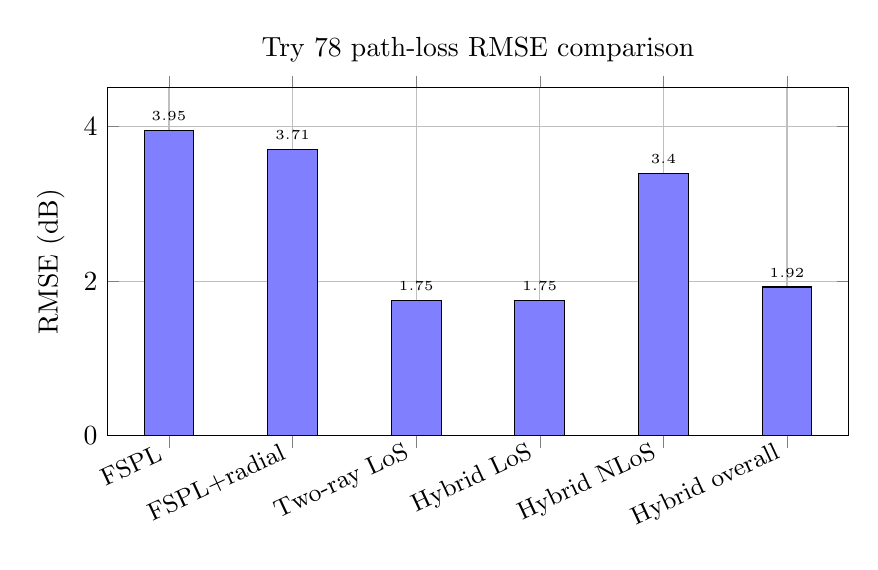
\begin{tikzpicture}
\begin{axis}[
  ybar, width=11cm, height=6cm, bar width=18pt,
  ylabel={RMSE (dB)},
  symbolic x coords={FSPL,FSPL+radial,Two-ray LoS,Hybrid LoS,Hybrid NLoS,Hybrid overall},
  xtick=data,
  x tick label style={rotate=25, anchor=east, font=\small},
  ymin=0, ymax=4.5,
  nodes near coords, nodes near coords align={vertical},
  every node near coord/.append style={font=\tiny},
  grid=major, title={Try 78 path-loss RMSE comparison}
]
\addplot[fill=blue!50] coordinates {
  (FSPL,3.9540)(FSPL+radial,3.7086)(Two-ray LoS,1.7516)
  (Hybrid LoS,1.7516)(Hybrid NLoS,3.3967)(Hybrid overall,1.9246)
};
\end{axis}
\end{tikzpicture}
\caption{Try 78 pixel-weighted RMSE values. The coherent two-ray model reduces LoS RMSE from 3.95~dB (FSPL) to 1.75~dB, a gain of 2.2~dB.}
\label{fig:try78_rmse}
\end{figure}

\begin{figure}[H]
\centering
\begin{tikzpicture}[
    >=stealth,
    node distance=1cm and 2cm,
    block/.style={draw, thick, fill=blue!10, rectangle, rounded corners, minimum width=3.5cm, minimum height=1cm, align=center},
    input/.style={draw, thick, fill=gray!20, rectangle, minimum width=2.5cm, minimum height=0.8cm, align=center},
    sum/.style={draw, thick, fill=green!10, rectangle, rounded corners, minimum width=3.5cm, minimum height=1cm, align=center},
    branch/.style={draw, thick, fill=orange!10, rectangle, rounded corners, minimum width=3.5cm, minimum height=1cm, align=center}
]
\node[input] (geom) {Geometry \\ $d_{2D}, \theta, h_{\mathrm{tx}}, h_{\mathrm{rx}}$};
\node[input, right=4cm of geom] (map) {CKM Map \\ $b(x), g(x), m_{\mathrm{LoS}}(x)$};
\node[block, below left=1.5cm and 0.5cm of geom] (fspl) {FSPL \\ (Eq.~\ref{eq:fspl_detail})};
\node[block, below=1.5cm of fspl] (tworay) {Coherent Two-Ray \\ $C_{\mathrm{2ray}}(x)$};
\node[block, below=1.5cm of tworay] (bias_rad) {Bias + Radial Residual \\ $b + r(d_{2D})$};
\node[branch, below=1.5cm of bias_rad] (pl_los) {Calibrated LoS \\ $\mathrm{PL}_{\mathrm{LoS}}(x)$};
\draw[->, thick] (geom.south) ++(-1,0) |- (fspl.east);
\draw[->, thick] (fspl) -- (tworay);
\draw[->, thick] (tworay) -- (bias_rad);
\draw[->, thick] (bias_rad) -- (pl_los);
\node[block, below right=1.5cm and 0.5cm of geom] (raw_nlos) {Raw NLoS Prior \\ $\max(\text{COST231}, \text{A2G})$};
\node[block, below=1.5cm of raw_nlos] (feat78) {Morphology Features \\ $\textbf{x}_{78}(x) \in \mathbb{R}^{15}$};
\node[block, below=1.5cm of feat78] (ols) {Regime-wise OLS \\ $\textbf{x}_{78}(x)^\top \hat{\textbf{w}}^{78}_{r}$};
\node[branch, below=1.5cm of ols] (pl_nlos) {Calibrated NLoS \\ $\mathrm{PL}_{\mathrm{NLoS}}(x)$};
\draw[->, thick] (geom.south) ++(1,0) |- (raw_nlos.west);
\draw[->, thick] (map.south) |- (feat78.east);
\draw[->, thick] (raw_nlos) -- (feat78);
\draw[->, thick] (feat78) -- (ols);
\draw[->, thick] (ols) -- (pl_nlos);
\node[sum, below right=1cm and 0.5cm of pl_los] (blend) {Switch on \\ $m_{\mathrm{LoS}}(x)$};
\node[input, below=1cm of blend] (final) {Hybrid Path Loss Prior \\ $\mathrm{PL}_{\mathrm{prior}}(x)$};
\draw[->, thick] (pl_los.south) |- (blend.west);
\draw[->, thick] (pl_nlos.south) |- (blend.east);
\draw[->, thick] (blend) -- (final);
\end{tikzpicture}
\caption{Pipeline for the \texttt{Try 78} hybrid path loss prior. The LoS branch relies on an explicit two-ray interference model, while the NLoS branch calibrates a raw prior against map-derived morphology features using regime-wise OLS.}
\label{fig:try78_pipeline}
\end{figure}
